\section{Context-Aware Weakly Supervised Network}
%%
%%
%%
%%
%%
%%
%%
%%
%%
%%
%%
%%
%%
%%
%%
%%
%%
%%
%%
%%
%%
%%
%%
%%
%%
%%
%%
%%
%%
%%
%%
%%
%%

In this section we describe our context-aware deep network for WSL.  Our network
consists of multiple CNN components, each of which builds on previous
models~\cite{Oquab:2015us,Girshick_2015_ICCV,Bilen:2015uo,Gidaris:2015cx}. We
begin by explaining first its overall architecture, and then detail our guidance
models for WSL.


\subsection{Overview}

Following the intuition of
Oquab~\etal\cite{Oquab:2015us}, our CNN-based approach to WSL learns a network from high-scoring object
candidate regions within a classification training setup. In this approach, the
visual consistency of classes within the dataset allows the network to localize
and learn the underlying objects. The overall network architecture is described
in Fig.~\ref{fig:model}.

\begin{figure}[t] 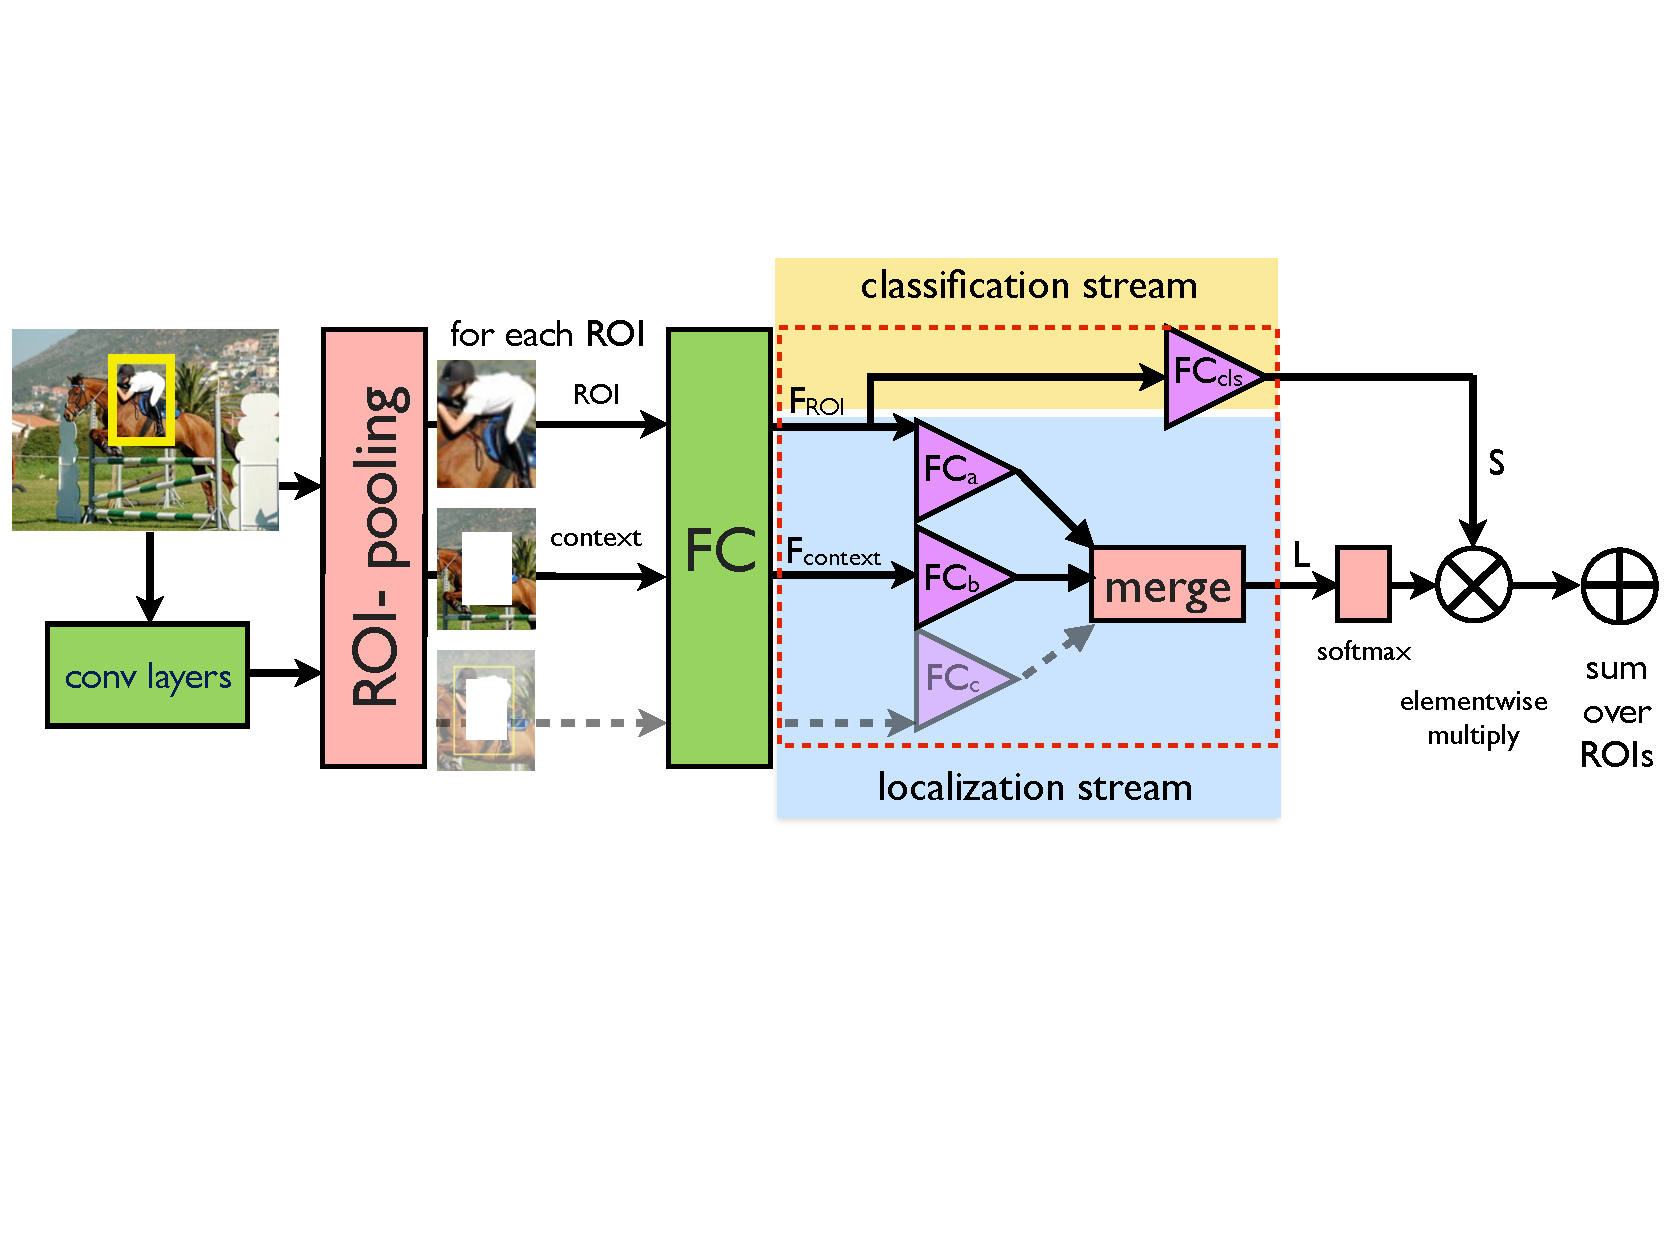
\includegraphics[width=\textwidth, trim={1mm 7.3cm 1mm 4cm},
clip]{eccv16_figures/model} \caption[Our context-aware architecture]{Our context-aware architecture. 
Convolutional layers and FC layers (in green) correspond to the VGG-F architecture, pre-trained on ImageNet.
%%
%%
The output of FC layers is passed through ReLu to the {\em classification} and {\em localization} streams. 
The classification stream takes features from ROIs, feeds them to a linear layer ${\rm FC_{cls}}$, and outputs classification scores ${\rm S_{ROI}}$. The localization stream takes features from ROIs and their context regions, processes them through our context-aware guidance models, and outputs localization scores ${\rm L_{ROI}}$. The final output is a product of classification and localization scores for each ROI and object class.
${\rm FC_{cls}}$, ${\rm FC_{a}}$, ${\rm FC_{b}}$, ${\rm FC_{c}}$ (in purple) are fully-connected linear layers trained from scratch. See text for more details.
%%
} 
\label{fig:model} 
\end{figure}


\subsubsection{Convolutional and ROI Pooling Layers.} 

Our architecture has 5 convolutional layers, followed by a ROI pooling
layer that extracts a set of feature maps, corresponding to the ROI (object
proposal). The convolutional layers, as our base feature extractor, come from
the VGG-F model~\cite{Chatfield14}. 
%%
%%
%%
%%
%%
 Instead of max pooling typically used to process output of the convolutional layers in conventional
CNNs for classification~\cite{Krizhevsky:2012wl,Oquab:2015us}, however, we
follow the ROI pooling of Fast R-CNN~\cite{Girshick_2015_ICCV}, an efficient
region-based CNN for object detection using object
proposals~\cite{uijlings2013selective}. This network first takes the
entire image as input and applies a sequence of convolutional layers resulting in feature maps (256 feature maps with the effective stride of 16 pixels). The network then contains a ROI-pooling
layer~\cite{He:2014wg}, where ROIs (object proposals) extract corresponding
features from the final convolutional layer. Given a ROI on the image and the
feature maps, the ROI-pooling module projects the ROI on the feature maps, pools
corresponding features with a spatially adaptive grid, and then forwards
them through subsequent fully-connected layers. This architecture allows us to
share computations in convolutional layers for all ROIs in an input image.
%%
%%
%%
%%
Following~\cite{Bilen:2015uo}, in this work, we initialize network layers using the weights of 
ImageNet-pretrained VGG-F model~\cite{Chatfield14}, which is then fine-tuned in training.

\subsubsection{Feature Pooling for Context-Aware Guidance.} For context-aware localization and
learning, we extend the ROI pooling by introducing additional pooling types 
for each ROI, in a similar manner to Gidaris~\etal\cite{Gidaris:2015cx}. 
As shown in Fig.~\ref{fig:roitransforms}, 
we define three types of pooling: ROI pooling, context pooling, and frame pooling. 
Given a ROI, \ie ~an object proposal~\cite{uijlings2013selective}, 
the {\it context} is defined as an outer region around the ROI, and the {\it frame} is an inner region ROI. Note that context pooling and frame pooling produce feature maps of the same shape, \ie central area of the outputs will have zero values. As will be explained in Sect.~\ref{sec:contrastive}, this property is useful in our contrast model.
The extracted feature maps are then independently
processed by fully-connected layers (green FC layers in Fig.~\ref{fig:model}), that outputs a ROI feature vector, a context feature vector, and/or a frame feature vector.   
The models will be detailed in Sects.~\ref{sec:additive}
and~\ref{sec:contrastive}. 

\begin{figure}[t] 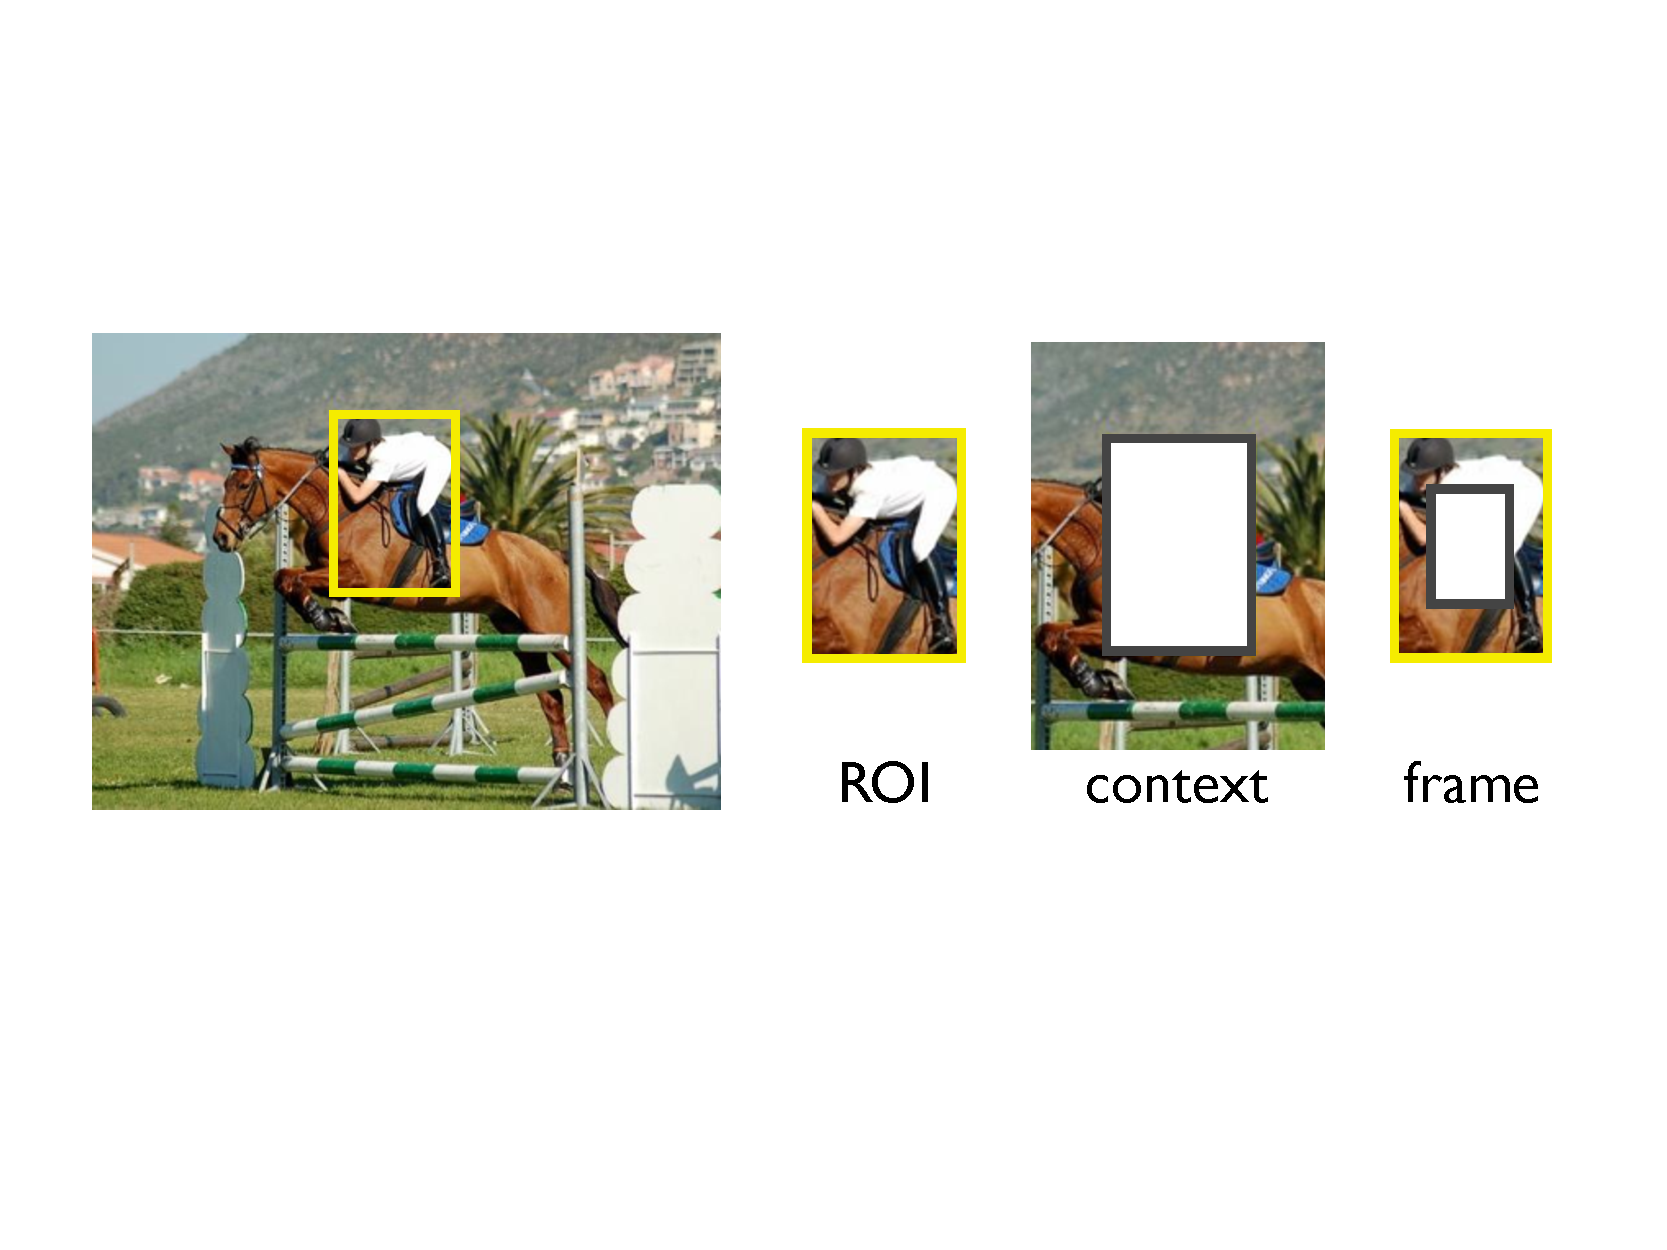
\includegraphics[width=\textwidth, trim={1mm 7.5cm 1mm 5cm},
clip]{eccv16_figures/roitransforms} \caption[Region pooling types for our guidance models]{Region pooling types for our guidance models: ROI pooling, context pooling, and frame pooling. For context and frame, the ratio between the side of the external rectangle and the internal rectangle is fixed as 
$1.8$. Note that context and frame pooling types are designed to produce feature maps of the same shape, \ie frame-shaped feature maps with zeros in the center.} \label{fig:roitransforms} \end{figure}



\subsubsection{Two-Stream Network.} To combine the guidance model components
with classification, we employ the two-stream architecture of Bilen and
Vedaldi~\cite{Bilen:2015uo}, which branches a localization stream in parallel
with a classification stream, and produces final classification scores by
performing element-wise multiplication between them. In this two-stream strategy, the
classification score of a ROI is reweighted with its corresponding softmaxed
localization score. As illustrated in Fig.~\ref{fig:model}, the {\em classification stream} takes the feature vector  
$F_{\rm ROI}$ as input and feeds it to a linear layer ${\rm FC_{cls}}$, that outputs a set of class
scores $S$. Given $C$ classes, processing $K$ ROIs produces a matrix $S \in \mathbb{R}^{K \times C}$. The {\em localization stream} takes $F_{\rm ROI}$ and $F_{\rm context}$ as inputs, processes them through our guidance models, giving a matrix of localization
scores $L \in \mathbb{R}^{K \times C}$. $L$ is then fed to a softmax layer $ [ \sigma(L) ]_{kc} = \frac{\exp(L_{kc})}{\sum_{k'=1}^{K}{\exp(L_{k'c})}}$ which normalizes the localization scores over the ROIs in the image. 
The final score for each ROI and class is obtained by element-wise multiplication of the corresponding scores $S$ and $\sigma(L)$. 
%%


This procedure is done for each ROI and, as a final step, we sum all the ROI
class scores to obtain the image class scores. During training, we use the hinge
loss function and train the model for multi-label image classification: $$L(w) =
\frac{1}{C \cdot N}\sum_{c=1}^{C}\sum_{i=1}^{N}\max(0, 1 - y_{ci} \cdot f_c(x_i;
w)),$$ where $f_c(x; w)$ is the score of our model evaluated on input image $x$
pararmeterized by $w$ (all weights and biases) for a class $c$; $y_{ci} = 1$ if
$i$'th image contains a ground truth object of class $c$, otherwise $y_{ci} =
-1$. Note that the loss is normalized by the number of classes $C$ and the
number of examples $N$. 




\subsection{Additive Model} \label{sec:additive}

%%
%%
%%
%%
%%
%%
%%
%%
%%
%%
%%
%%
%%
%%
%%
%%
%%
%%
%%
%%

The additive model, inspired by the conventional use of contextual
information~\cite{Oliva:2007ui,Rabinovich:2007wy,Felzenszwalb:2009wx,Girshick:2016ig,Gidaris:2015cx},
encourages the network to select a ROI that is semantically compatible with its context. 
Specifically, we introduce two fully-connected layers ${\rm FC_{ROI}}$ and ${\rm FC_{context}}$ as shown in Fig.~\ref{fig:models} (a), and the localization score for each ROI is obtained by summing outputs of the layers. Note that compared to context-padding~\cite{Girshick:2016ig}, 
this model separates a ROI and its
context, and learns the adaptation layers ${\rm FC_{ROI}}$ and ${\rm
FC_{context}}$ in different branches. This conjunction of separate
branches allows us to learn context-aware activations for the ROI in an
effective way. %%
%%
%%

Figure~\ref{fig:modelvis}(top) illustrates the behavior of the ${\rm FC_{ROI}}$ and ${\rm FC_{context}}$
branches of the additive model trained on PASCAL VOC 2007. The scores of
the target object (car) vary for different sizes of object proposals.
We observe that the ${\rm FC_{context}}$ branch discourages small detections on the
interior of the object as well as large detections outside of object boundaries.
${\rm FC_{context}}$ is, hence, complementary to ${\rm FC_{ROI}}$ and can be expected to prevent detections
outside of objects.

%%
%%
%%

%%
%%
%%
%%

%%
%%

%%
\begin{figure}[t] 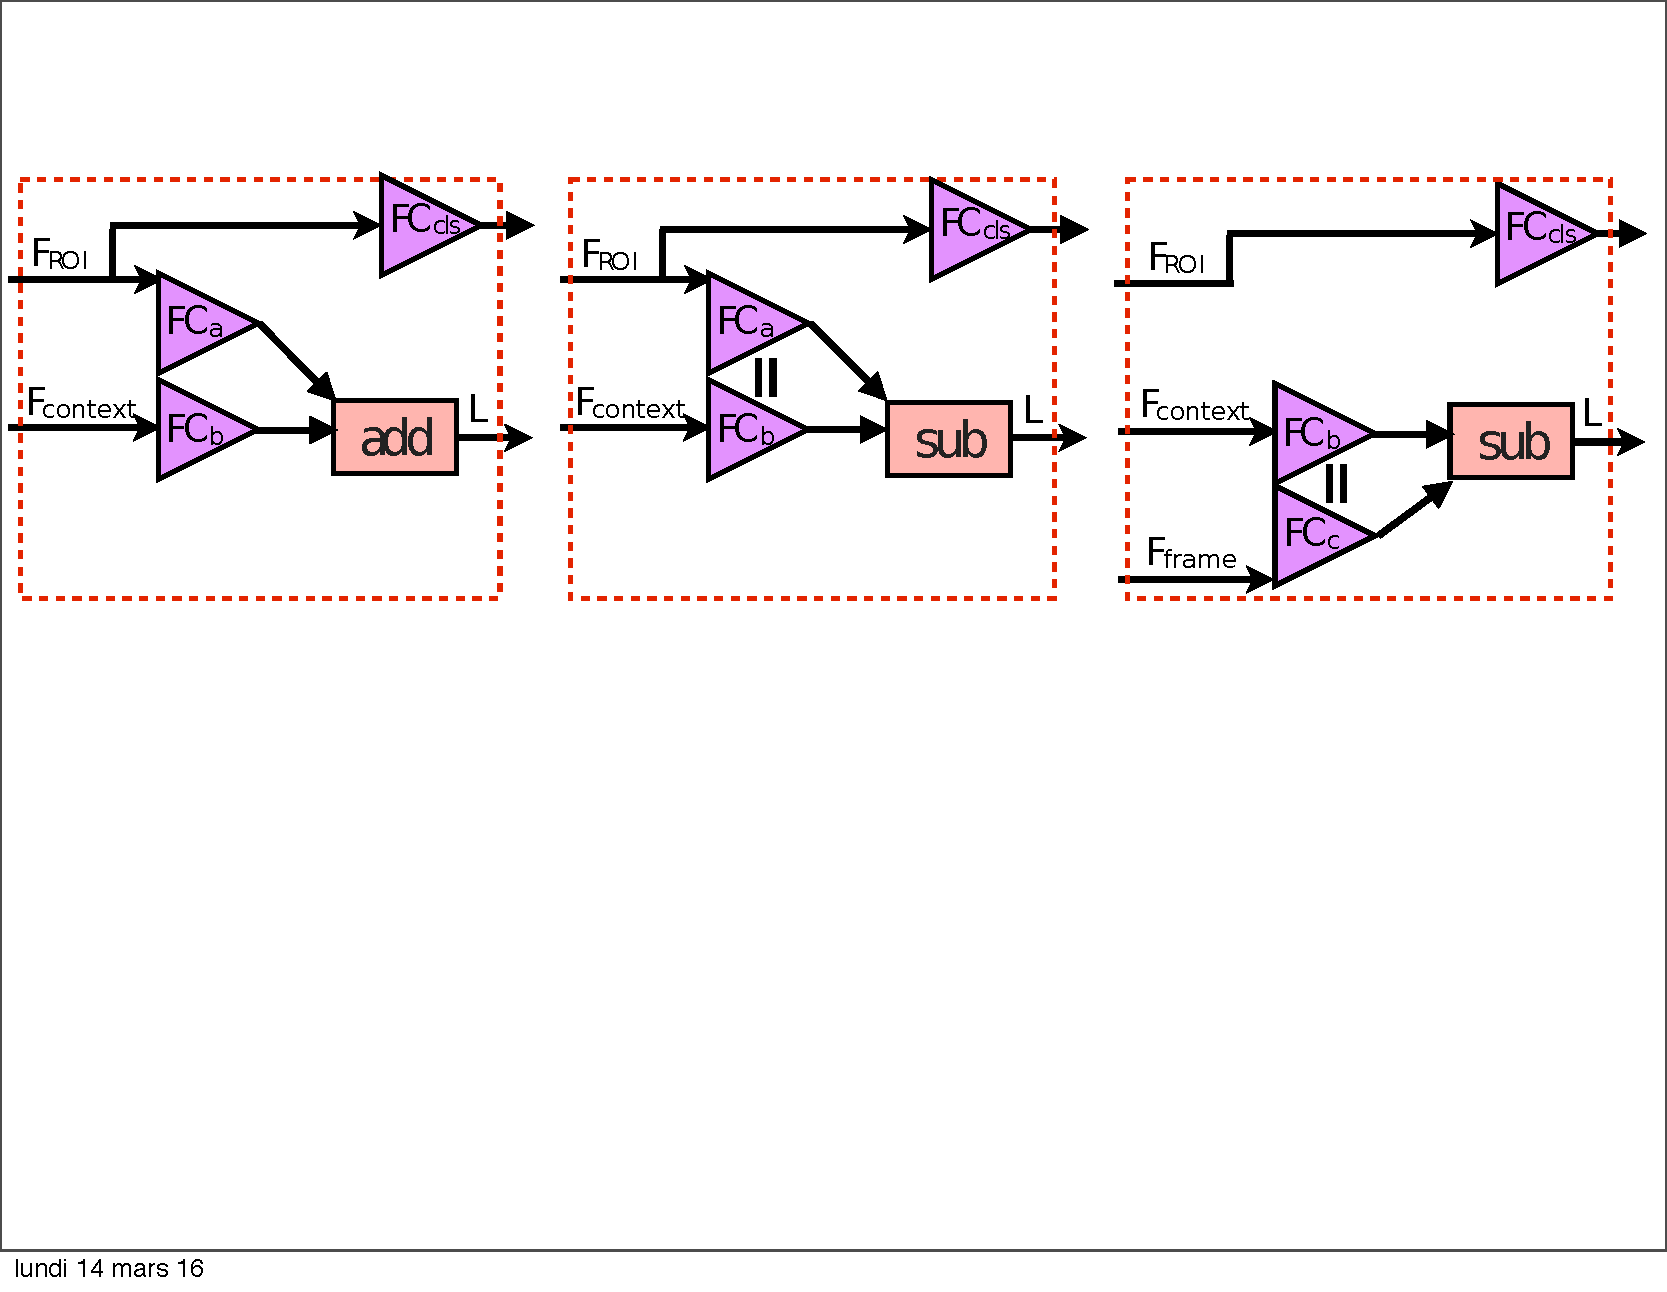
\includegraphics[width=\textwidth, trim={2mm 11.5cm 2mm 3cm},
clip]{eccv16_figures/variants-horiz} \begin{minipage}{0.32\linewidth} \centering
\small{(a) Additive model. } \end{minipage} \begin{minipage}{0.32\linewidth}
\centering \small{(b) Contrastive model A. } \end{minipage}
\begin{minipage}{0.32\linewidth} \centering \small{(c) Contrastive model S. }
\end{minipage}
\caption[Context-aware guidance models]{Context-aware guidance models.
The additive model takes outputs of ROI and context pooling, feeds them to independent fully-connected layers, and compute localization scores by adding their outputs.  
The contrastive models take outputs of ROI (or frame) and context pooling, feed them to a shared fully-connected layer (\ie~two fully-connected layers with all parameter shared), and compute localization scores by subtracting the output of context from the other. For details, see the text.}
\label{fig:models} \end{figure}




\begin{figure}[t]
\centering
%%
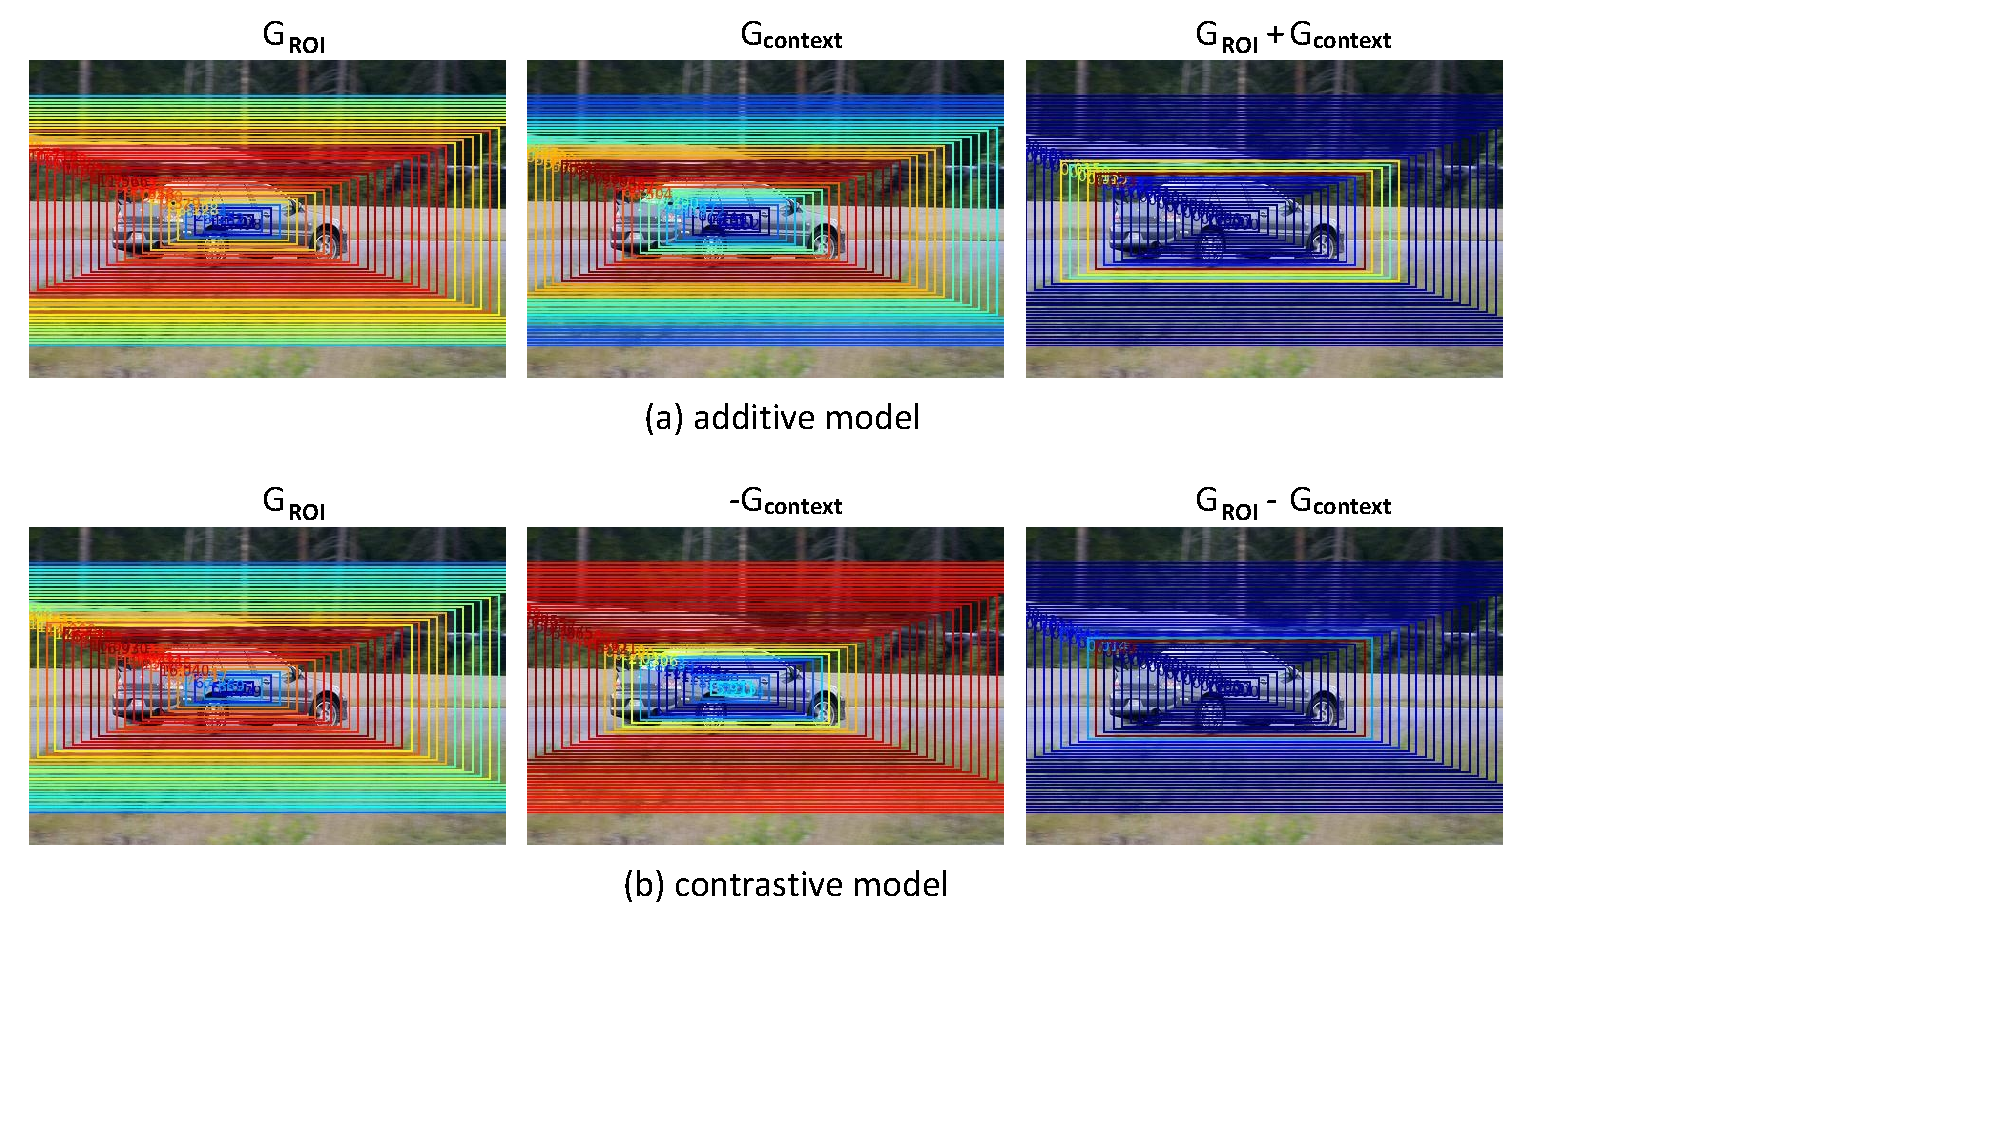
\includegraphics[width=\textwidth, trim={0mm 3.5cm 8cm 0cm},clip]{eccv16_figures/modelvis.pdf}
\caption[Visualization of object scores produced by different branches of our models]{
Visualization of object scores produced by different branches of our models. The scores are computed
for the {\em car} class for bounding boxes of different sizes centered on the target object. Red and blue
colors correspond to high and low scores respectively. While the outputs of ${\rm FC_{ROI}}$ branches for the
additive and contrastive models are similar, the ${\rm FC_{context}}$ branches, corresponding to feature
pooling at object boundaries, have notably different behavior. The ${\rm FC_{context}}$ branch of the additive model
discourages detections outside of the object. The ${\rm FC_{context}}$ branch of the contrastive model, discourages
detections on the interior of the object. The combination of the ${\rm FC_{ROI}}$ and ${\rm FC_{context}}$ branches results in correct object
localization for both models.
}
\label{fig:modelvis}
\end{figure}

\subsection{Contrastive Model} \label{sec:contrastive}
%%
%%
%%
%%
%%
%%
%%
%%
%%
%%
%%
%%
%%
%%
%%
%%

%%
%%


The contrastive model encourages the network to select a ROI that is
outstanding from its context.  This model is inspired by Cho~\etal's
standout scoring for unsupervised object discovery~\cite{Cho:2015vz}, which
measures the maximum contrast of matching scores between a rectangular box and
its surrounding boxes. We adapt this idea of semantic contrast to our ROI-based
CNN architecture. Specifically, we introduce two fully-connected layers ${\rm FC_{ROI}}$ and ${\rm FC_{context}}$ as shown in Fig.~\ref{fig:models} (b), and the locacalization score for each ROI is obtained by subtracting the output activation of ${\rm FC_{context}}$ from that of ${\rm FC_{ROI}}$ for each ROI.
Note that in order to make subtraction work properly, all weights of the layers ${\rm
FC_{ROI}}$ and ${\rm FC_{context}}$ are shared for this model. Without sharing parameters, this model reduces to the additive model.  %%
%%
%%
%%

Figure~\ref{fig:modelvis}(bottom) illustrates the behavior of ${\rm FC_{ROI}}$ and ${\rm FC_{context}}$
branches of the contrastive model. We denote by $G_{\rm ROI}$ and $G_{\rm context}$ the outputs of respective layers. The variation of scores for the car object
class and different object proposals indicates low responses of $-G_{\rm context}$
on the interior of the object. The combination $G_{\rm ROI}-G_{\rm context}$ compensate each other
resulting in correct localization of object boundaries. We expect the
contrastive model to prevent incorrect detections on the interior of the object.

One issue in this model is that in the localization stream the shared adaptation layers ${\rm FC_{ROI}}$ and ${\rm FC_{context}}$ need to process input feature maps of different shapes ${\rm F_{ROI}}$ and ${\rm F_{context}}$, \ie  ${\rm FC_{ROI}}$ processes features from a whole region ({\em ROI} in Fig. \ref{fig:roitransforms}), whereas ${\rm FC_{context}}$ processes features from a frame-shaped region ({\em context} in Fig. \ref{fig:roitransforms}). We call this model the asymmetric contrastive model ({\em contrastive A}).  

To remove this asymmetry in the localization stream, we replace ROI pooling with {\em frame} pooling (Fig.~\ref{fig:roitransforms}) that extracts a feature map from an internal rectangular frame of ROI. This allows the shared adaptation layers in the localization stream to process input feature maps of the same shape ${\rm F_{frame}}$ and ${\rm F_{context}}$. We call this model the symmetric contrastive model ({\em contrastive S}). Note that adaptation layer ${\rm
FC_{cls}}$ in the classification stream maintains the original ROI pooling 
regardless of modification in the localization stream. The advantage of this
model will be verified in our experimental section.  

